%%%%%%%%%%%%%%%%%%%%%%%%%%%%%%%%%%%%%%%%%%%%%%%%%%%%%%%%%
%%%
%%%  Chapter 1
%%%  Introduction
%%%
%%%%%%%%%%%%%%%%%%%%%%%%%%%%%%%%%%%%%%%%%%%%%%%%%%%%%%%%%
In the ambitious pursuit of lunar exploration, the traditional boundaries of robotics are being redefined. The quest for a robot capable of navigating the hazardous lunar environment has led to the development of Moonbot, a modular legged robot designed to transcend the limitations of conventional rover-based exploration. The essence of Moonbot lies in its ability to dynamically adapt and respond to the challenges presented by the lunar terrain.\\

%%%%% BACKGROUND %%%%%
\section{Background}\label{sec:background}
\indent
Lunar exploration has long captured the imagination of humanity. From the Apollo missions \cite{apollo} of the 20th century to the more recent lunar rovers, our quest to uncover the secrets of the Moon has driven technological innovation and expanded our understanding of space.

As we look towards the future, the vision of establishing a permanent human presence on the Moon looms ever larger. Central to this vision is the construction of lunar bases, which will serve as hubs for scientific research, and resource utilization, and even as launch pads for missions deeper into space. However, the harsh and unforgiving lunar environment presents formidable challenges for such endeavors.

\begin{figure}[h]
  \centering
  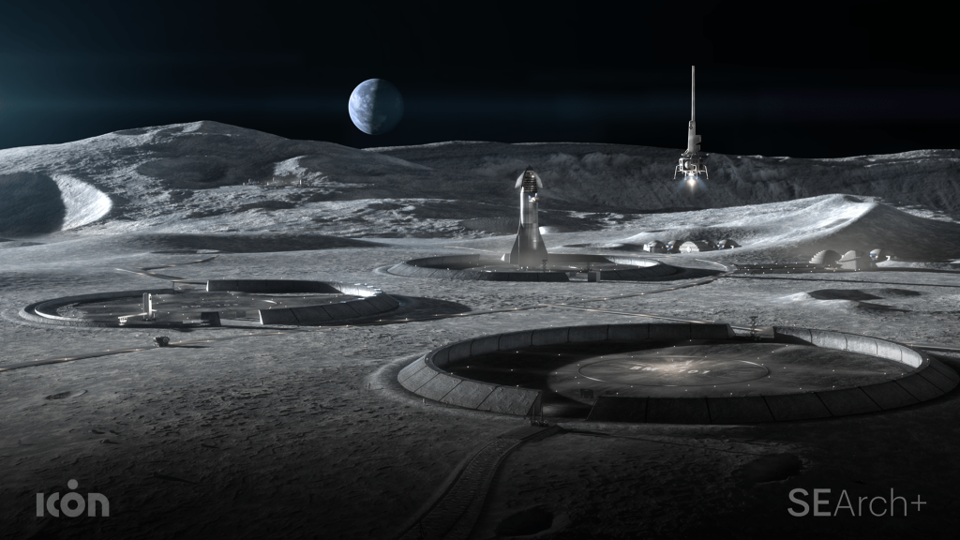
\includegraphics[width=140mm]{./fig/intro/lunarconstruct.png}
  \vspace{2mm}
  \caption{NASA’s Moon to Mars Autonomous Construction Technologies project to advance space-based construction capabilities for long-duration exploration missions on the Moon or Mars. \cite{nasa_construct}}\label{lunar construct}
\end{figure}

In the realm of space robotics research, modular robots, \cite{modularity}, \cite{electrovoxel} emerge as a transformative concept, reshaping our approach to space exploration. A modular robot is a versatile robotic system composed of interchangeable and reconfigurable modules that can be assembled in various configurations to adapt to different tasks and environments. Modular robots have been introduce to space robotics \cite{worms} marks a significant shift, providing unprecedented flexibility and adaptability for the challenges posed by extraterrestrial terrains.

In this thesis, we explore the development and capabilities of Moonbot, a modular legged robot designed for lunar exploration and base construction, following the target of Moonshot Project, Self-evolving AI Robot System for Lunar Exploration and Human Outpost Construction \cite{moonshotGoal3B}. Through a combination of advanced control algorithms, Moonbot aims to push the boundaries of what is possible in extraterrestrial robotics. By harnessing the power of modular design and cutting-edge technology, we strive to pave the way for a new era of lunar exploration and human settlement.
%%%%% BACKGROUND %%%%%

%%%%% LEGGED vs WHEELED %%%%%
\section{Legged vs Wheeled}
Researchers are increasingly considering a shift from wheeled to legged robotic system \cite{spacebok}, particularly in environments where the terrain presents uncertainties. Although wheeled vehicles dominate exploration beyond Earth, this trend might be evolving. While wheels are effective on celestial bodies like the Moon and Mars, other challenging environments, such as smaller moons and asteroids, demand more adaptable solutions. In these low-gravity settings, robots navigating uneven terrain face the possibility of entering prolonged flight phases, a potentially hazardous situation for robots unprepared for such conditions. Below, we explore some of these advantages.\\

\begin{figure}[h]
  \centering
  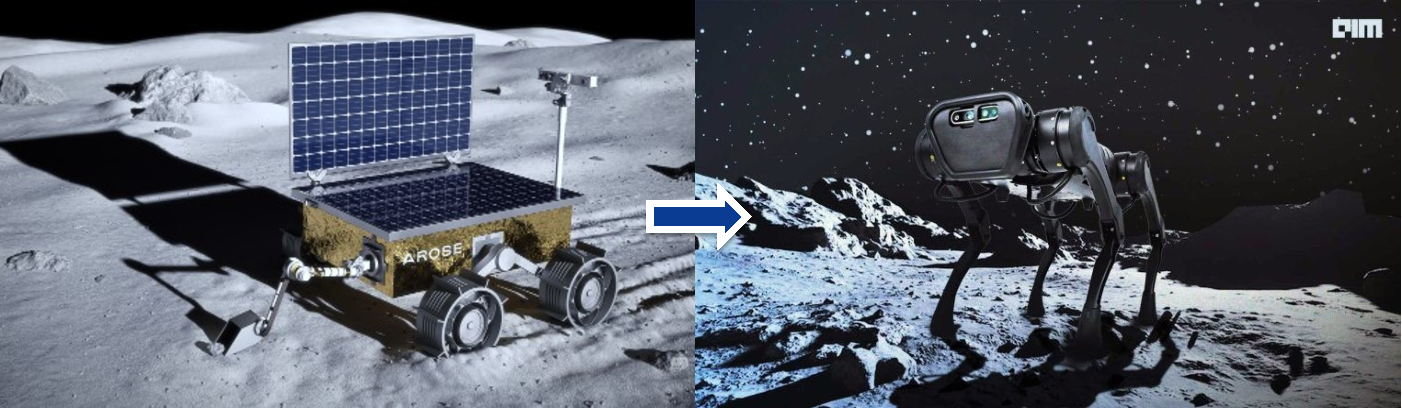
\includegraphics[width=150mm]{./fig/intro/leggedvswheeled.pdf}
  \vspace{2mm}
  \caption{Development of space rover and space legged robot.}\label{fig1}
\end{figure}

\subsection{Mobility}
Legged robots offer superior mobility compared to wheeled robots due to their inherent omni-directional nature. This means that a legged robot can alter its direction independently of the main body axis simply by adjusting its footholds. In contrast, a traditional wheeled robot would need to perform specific maneuvers to change its direction.

Moreover, a legged robot can manipulate its body's movement and orientation while preserving footholds through adjustments in leg extension. This characteristic grants the robot an additional six degrees of freedom (DOF) for its body. It's important to note that while a wheeled robot with traction and directional motors can enhance its directionality, this often comes with the drawback of increased system complexity. Some robots also utilize specialized wheels, such as the ilonator wheel \cite{omniwheel}, to achieve omnidirectionality, but this is typically effective only on flat surfaces.

\subsection{Overcoming Obstacles}
A legged robot has the capability to surmount obstacles situated below its maximum ground clearance by stepping on them. In contrast, a wheeled robot can only navigate obstacles with heights up to half of its wheel radius \cite{mckerrow}. Tracks, which are composed of a virtual wheel with a radius equal to half the track length, allow tracked vehicles to overcome higher obstacles compared to wheeled ones, albeit requiring substantial body motions.

\subsection{Active Suspension}
A legged robot inherently incorporates an active suspension system by adjusting the lengths of its legs in response to terrain irregularities. This capability enables a legged robot to traverse highly uneven terrain while maintaining a level body, ensuring smooth and comfortable motion for riders. In contrast, a wheeled robot keeps its body parallel to the terrain and experiences comparable tilts to the ground.

\subsection{Natural Terrain}
Wheeled vehicles demand costly, consistently paved surfaces for efficient movement. In contrast, legged systems, in principle, do not necessitate prepared terrain like their wheeled counterparts. They can navigate sandy, muddy, rigid, and soft terrains with comparable efficiency. Additionally, legged systems do not rely on continuous terrain for movement, providing another advantage.

\subsection{Slippage and Jamming}
Wheeled vehicles often encounter difficulties moving in soft terrain as their wheels tend to sink. In contrast, a leg, when placed vertically on the ground, only compresses the soft ground in a single direction. Vertical leg lifting avoids interference with the ground, and when the body is in motion, the feet rotate around their joints, preventing legs from interacting with the ground and causing jamming issues. This holds true for vehicle slippage during forward or backward propulsion.

\subsection{Environment Damage}
Legged robots necessitate specific points of contact with the ground, whereas wheeled or tracked vehicles rely on continuous paths along the ground. As a result, legged robots have reduced ground contact compared to conventional vehicles, leading to diminished environmental impact.

%%%%% LEGGED vs WHEELED %%%%%

%%%%% Potential of Legged Robots for Planetary Exploration %%%%%
\section{Legged Robots for Planetary Exploration}
Legged robots' capability to navigate diverse and unknown terrains, surmount obstacles, and employ discrete ground contact points positions them as ideal candidates for planetary exploration. Specific robots have been purposefully designed and tested for such applications, including: (a) the AMBLER, created by Carnegie-Mellon University with NASA funding, serving as an experimental platform for technology development related to potential Mars missions \cite{bares}.\\

\begin{figure}[h]
  \centering
  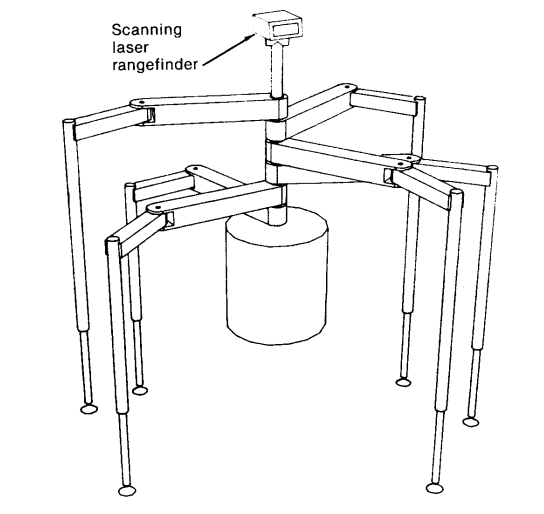
\includegraphics[width=70mm]{./fig/intro/ambler.png}
  \vspace{2mm}
  \caption{Sketch of the AMBLER robot. \cite{bares}}\label{fig ambler}
\end{figure}
%%%%% Potential of Legged Robots for Space Exploration %%%%%

%%%%% Modular Robot %%%%%
\section{Modular Robots: Versatile Solutions for Robotics}

Modular robots represent a fascinating approach to robotics design, offering versatility, adaptability, and scalability in various applications. These robots consist of individual modules or units that can be reconfigured and assembled into different shapes and configurations to suit specific tasks and environments. This modular design allows for flexibility in robot morphology, enabling robots to adapt to diverse operating conditions and perform a wide range of tasks.

\begin{itemize}
    \item \textbf{Versatility}: Modular robots can be reconfigured into various shapes and configurations, allowing them to adapt to different tasks and environments.
    
    \item \textbf{Adaptability}: The ability to dynamically adjust robot morphology enables modular robots to traverse diverse terrain, navigate obstacles, and access hard-to-reach areas.
    
    \item \textbf{Scalability}: Modular design facilitates scalability, allowing robots to be easily expanded or downsized by adding or removing modules as needed.
    
    \item \textbf{Redundancy and Fault Tolerance}: Modular robots inherently offer redundancy and fault tolerance, as module failure or damage can be mitigated by redistributing or replacing modules.
    
    \item \textbf{Resilience}: The ability to reconfigure and adapt to changing conditions enhances the resilience of modular robots, making them suitable for operation in remote and hazardous environments.
\end{itemize}

% In the context of space exploration, where the environment is often harsh, unpredictable, and challenging to navigate, modular robots hold significant promise. The ability to reconfigure robot morphology on-demand can be particularly advantageous for traversing uneven terrain, navigating obstacles, and accessing hard-to-reach areas. By adjusting their configuration, modular robots can optimize their locomotion capabilities to suit the terrain, whether it's rocky, sandy, or steep.

% The lunar surface, with its rugged terrain and varied topography, presents numerous challenges for robotic exploration. Modular robots offer a compelling solution for lunar exploration missions, as their adaptable design allows them to navigate the lunar landscape with agility and resilience. By reconfiguring their morphology to match the terrain, modular robots can traverse crater-like surfaces, scale rocky inclines, and explore lunar caves and crevices.

Moonbot, our modular legged robot designed for space exploration, exemplifies the synergy between modular robotics and lunar exploration. Equipped with a modular architecture, Moonbot is a significant prototype for future lunar exploration mission.

In the event of module failure or damage, the robot can dynamically reconfigure itself by redistributing or replacing modules, ensuring continuity of operation and mission success.

In summary, modular robots represent a paradigm shift in robotics design, offering unparalleled versatility, adaptability, and resilience for lunar exploration and beyond. With their ability to navigate challenging terrain and withstand harsh environmental conditions, these robots hold immense potential to advance our understanding of the Moon and pave the way for future human exploration and habitation.

\begin{figure}[t]
    % \begin{subfigure}{0.45\textwidth}
    %     \centering
    %     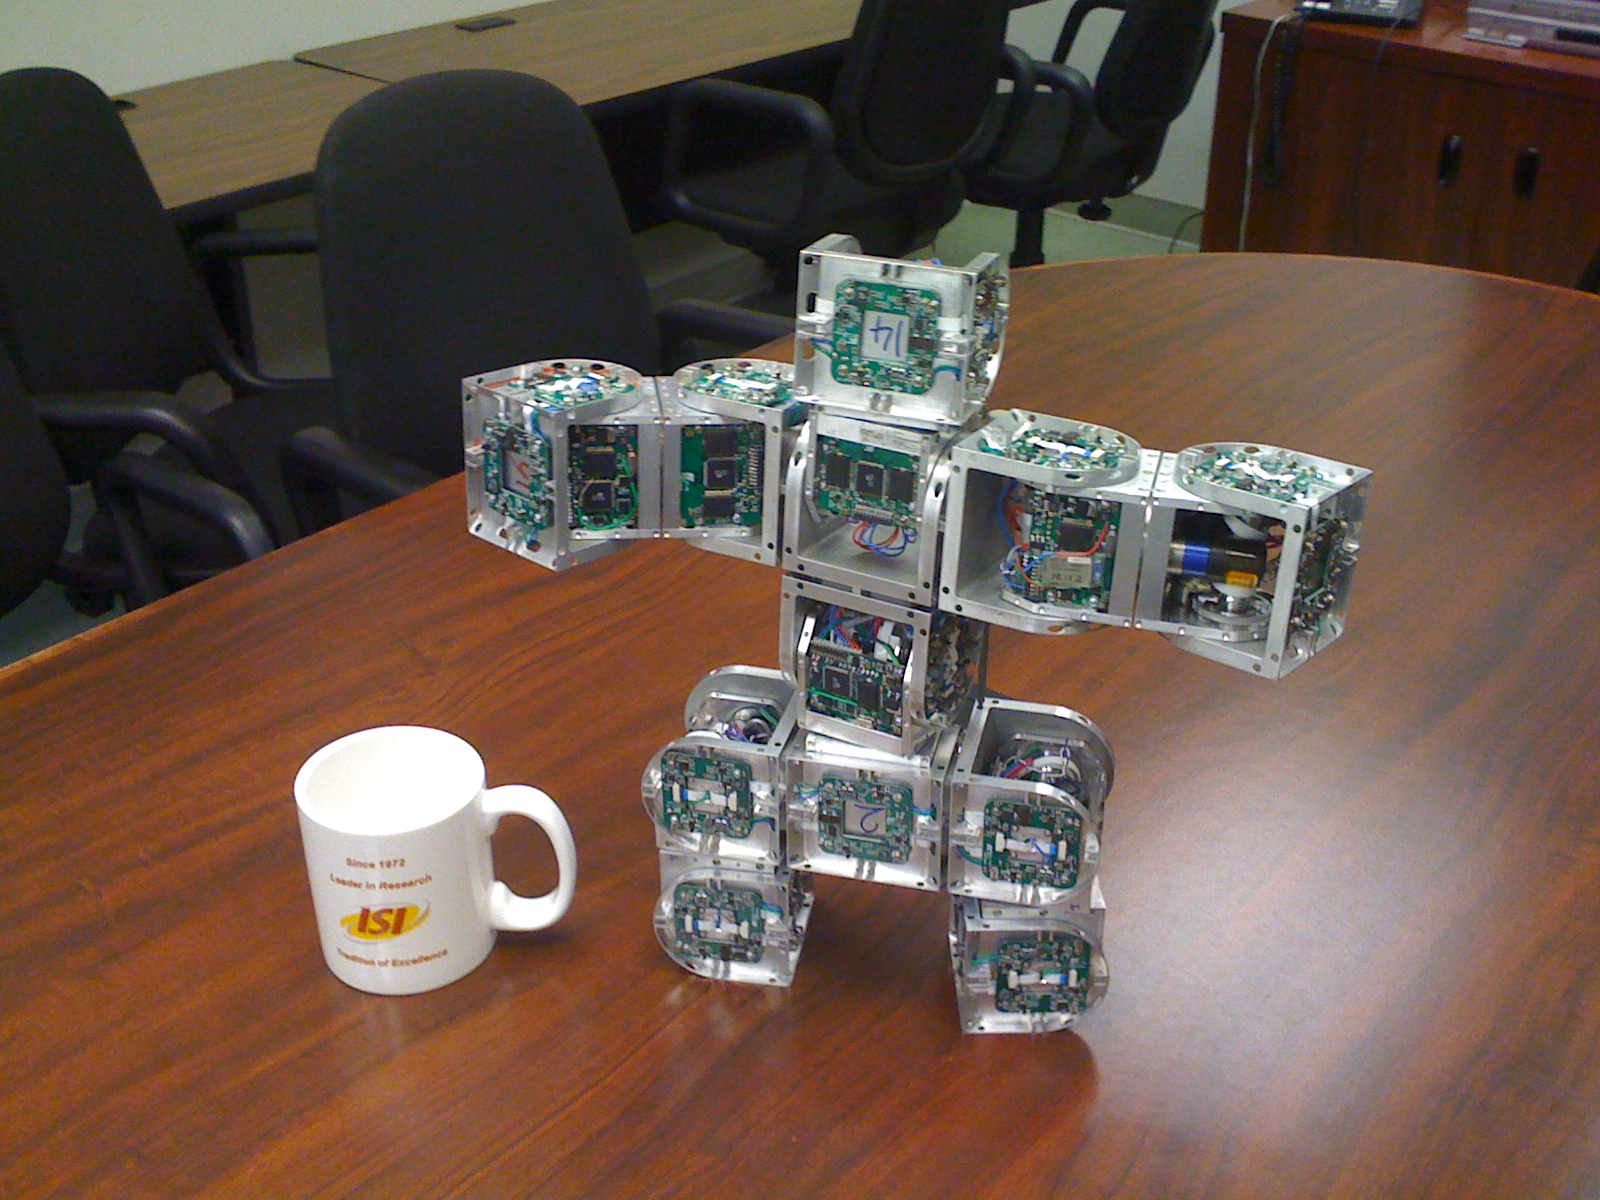
\includegraphics[height=40mm]{./fig/intro/modularrobot/SuperBotCup.jpeg}
    %     \caption{Superbot the modular robot. \cite{Superbot}}
    %     \label{superbot}
    % \end{subfigure}
    % \hfill
    \begin{subfigure}{1.0\textwidth}
        \centering
        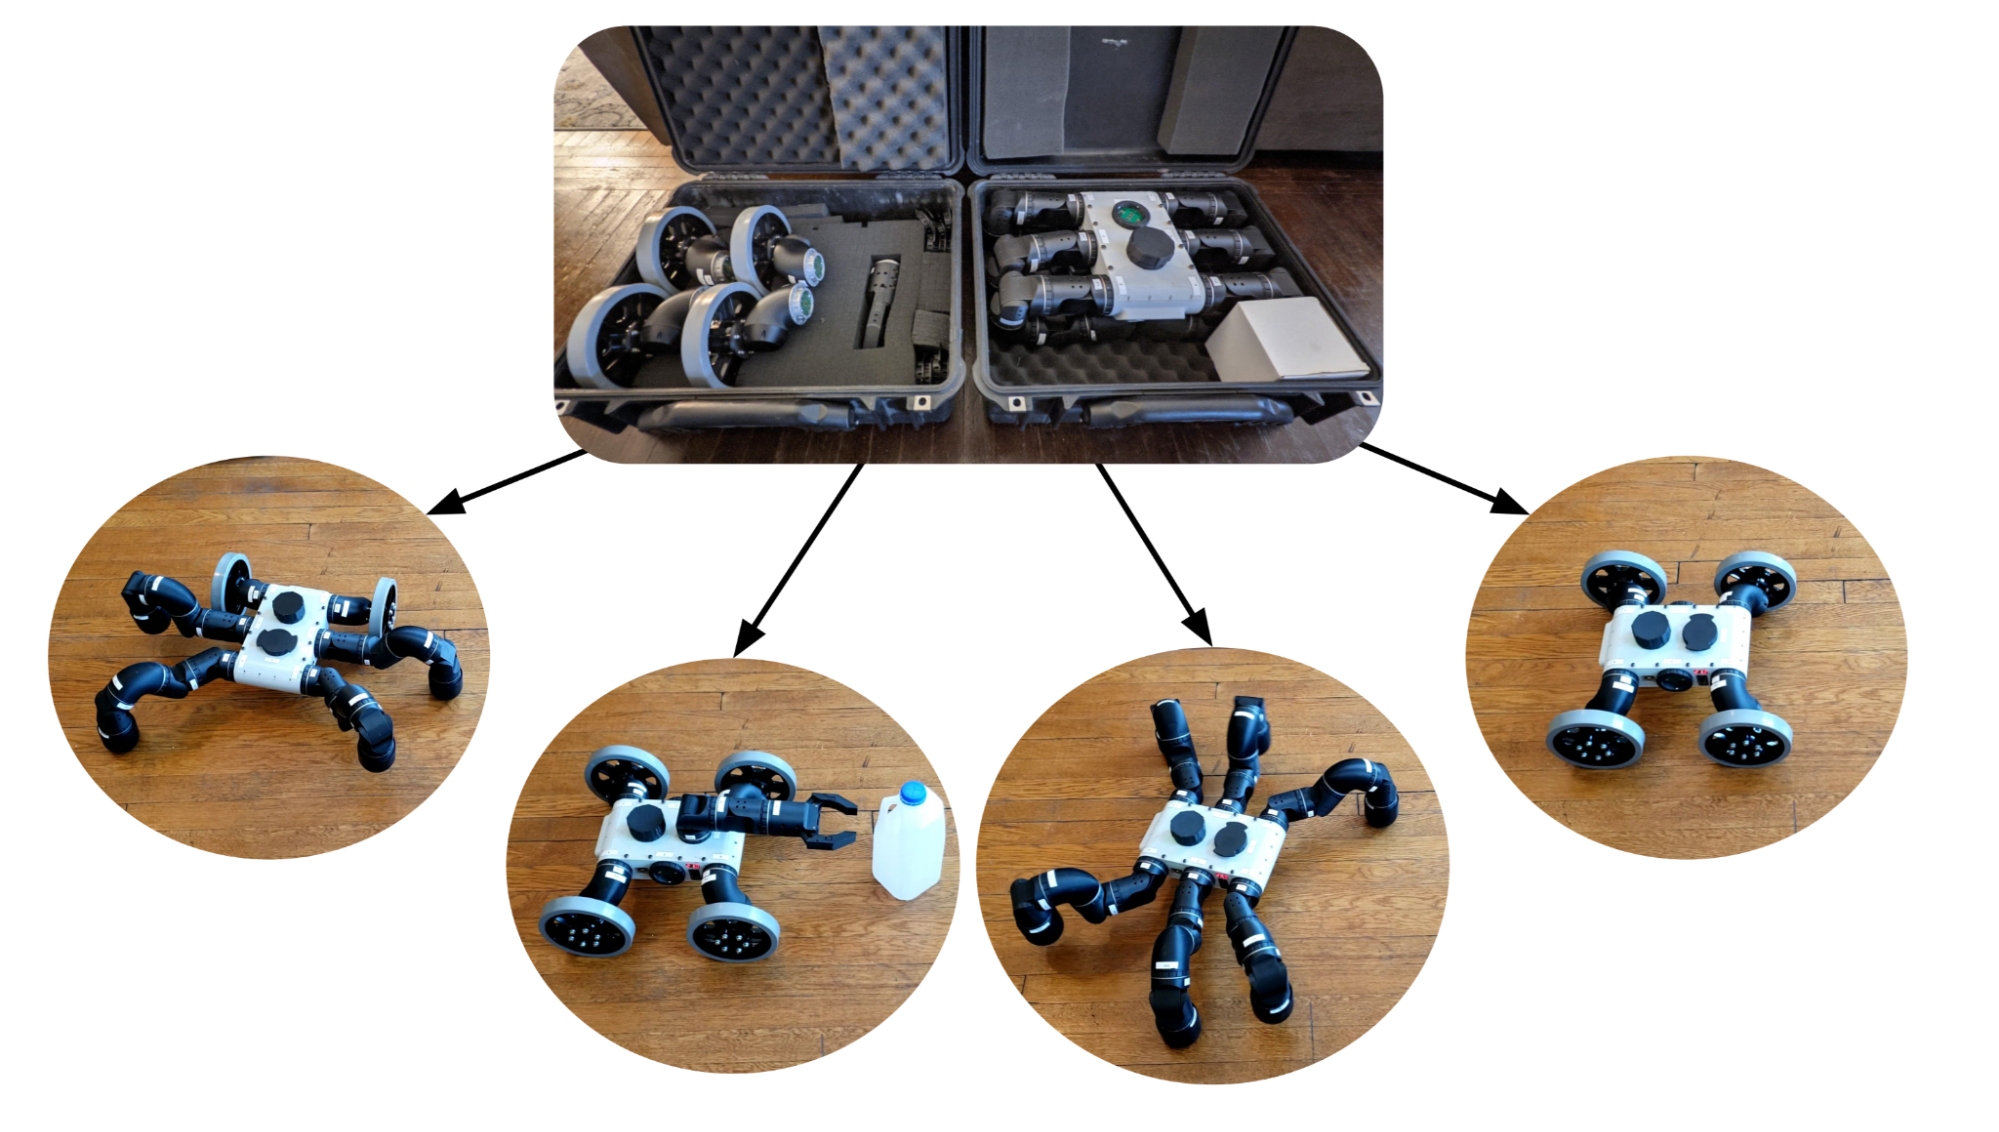
\includegraphics[height=52mm]{./fig/intro/modularrobot/Eigenbot.png}
        \caption{Superbot’s modular units self-assemble. \cite{Eigenbot}}
        \label{Eigenbot}
    \end{subfigure}
    \begin{subfigure}{0.45\textwidth}
        \centering
        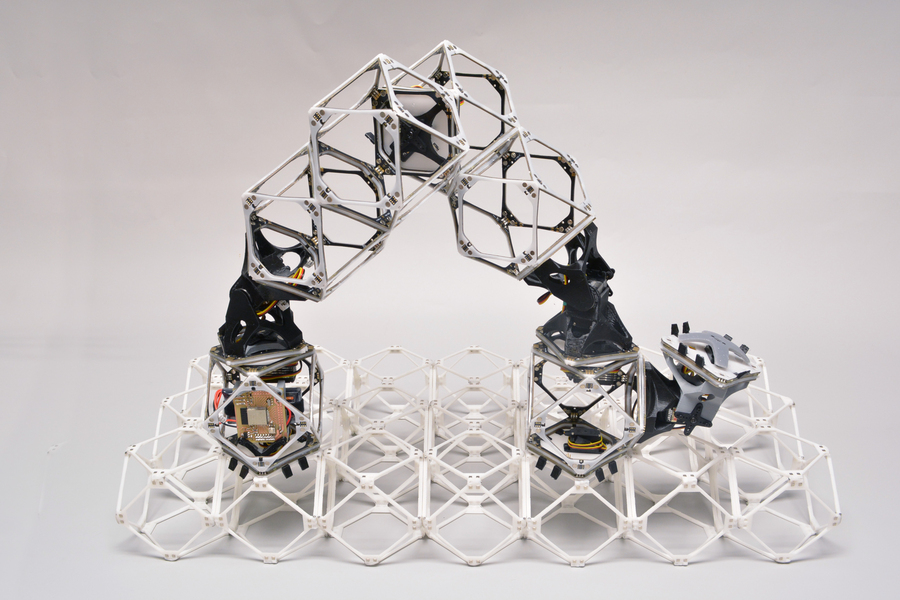
\includegraphics[height=52mm]{./fig/intro/modularrobot/MIT-Robot.jpg}
        \caption{Assembler bot from MIT. \cite{MITassembler}}
        \label{MITbot}
    \end{subfigure}
    \hfill
    \begin{subfigure}{0.45\textwidth}
        \centering
        \includegraphics[height=52mm]{./fig/intro/modularrobot/snap-bot.jpg}
        \caption{Snapbot the modular legged robot. \cite{snapbot1}}
        \label{snapbot}
    \end{subfigure}
    \vspace{2mm}
    \caption{Examples of modular robots.}
    \label{modular-robot}
\end{figure}


%%%%% Modular Robot %%%%%

%%%%% MOONSHOT PROJECT %%%%%
\section{Moonshot Project}
The Moonshot project of the Space Robotics Laboratory, led by Prof. Kazuya Yoshida at Tohoku University, aims to accomplish Goal 3: ``Realization of AI robots that autonomously learn, adapt to their environment, evolve in intelligence, and act alongside human beings by 2050" \cite{moonshotproject}. In alignment with this goal, the project envisions the development of a ``Self-evolving AI Robot System for Lunar Exploration and Human Outpost Construction"\cite{moonshotGoal3B}. The project has identified several key objectives to achieve this vision:
\vspace{1mm}
\begin{enumerate}
    \item Design modular and reconfigurable heterogeneous robotic systems.
    \item Develop a transferable AI system for plug-and-play implementation.
    \item Enable on-demand robot design and on-site assembling capabilities.
\end{enumerate}

As part of the Moonshot project, our team has developed ``Moonbot", a modular robot designed to address the challenges of lunar exploration. Moonbot inherits the vision of the Moonshot project, integrating autonomous learning, adaptability, and intelligence. This modular robot represents a pioneering step towards the project's overarching goal.

Moonbot draws inspiration from innovative modularity concepts in legged robotics, including the Snapbot project \cite{snapbot1} \cite{snapbot2}, as well as general modular robotics advancements \cite{modularrobot}. These projects laid the foundation for Moonbot's approach to modularity.

The advancement of Moonbot's design is the integration of modularity concept with a higher-level legged robot control system \cite{syropod}. This combination results in a robotic platform capable of self-recognition, adaptability, and dynamic selection of control motions. Moonbot inherits the ability to configure its legs dynamically, ranging from one to four, thus enhancing its versatility and locomotion capabilities.\\

\begin{figure}[t]
  \centering
  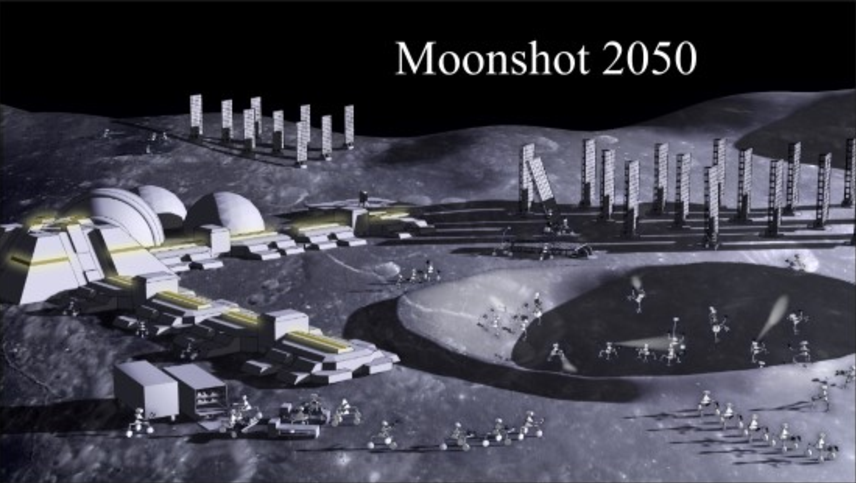
\includegraphics[width=\linewidth]{./fig/intro/moonshot.pdf}
  \vspace{2mm}
  \caption{lunar base with AI robots in 2050. \cite{moonshotGoal3B}}\label{fig moonshot}
\end{figure}
%%%%% MOONSHOT PROJECT %%%%%

%%%%% OBJ %%%%%
\section{Research Objectives}
This thesis aims to develop the first prototype of modular control system for legged robots. By using the implemented internal sensors, the robot can recognize the configuration and select the appropriate strategy of motion control, referred as self-recognition ability.

Secondly, the research aims to realize sophisticated software control mechanisms and high-level controllers for the quadruped modular robot. By designing and implementing robust software architectures, the robot can execute complex locomotion patterns. Through these objectives, the research endeavors to enhance the autonomy, adaptability, and overall performance of modular legged robots, paving the way for advancements in robotic exploration and deployment scenarios.\\
%%%%% OBJ %%%%%

% \section{Research Plan Proposal}
% The email address below is the author's contact information. We are always accepting bug reports and questions. \\
% \texttt{unoken@tohoku.ac.jp}

%%%%% OVERVIEW %%%%%
\section{Thesis Overview}
The structure of this thesis is outlined below. 

\begin{itemize}
    \item \textbf{Chapter 1: Introduction}: \\
    This chapter serves as an introduction to the thesis, providing background information and the purpose behind the research.
   
    \item \textbf{Chapter 2: Modular Legged Robot: "Moonbot"}: \\
    This chapter offers an in-depth exploration of Moonbot's structural composition, focusing on its hardware overview, modularity, and self-recognition capabilities.

    \item \textbf{Chapter 3: Software and Self-Recognition Algorithms}: \\
    Here, the thesis delves into the software architecture and logic of Moonbot's self-recognition algorithms, detailing the tools and methodologies used in their development.

    \item \textbf{Chapter 4: Motion Control}: \\
    This chapter examines Moonbot's motion control mechanisms, including its kinematics and locomotion strategies. It provides insights into how the robot navigates and moves within its environment.

    \item \textbf{Chapter 5: Conclusions}: \\
    The final chapter concludes the thesis with a summary of the achieved results, reflections on the challenges encountered, and proposals for future advancements in lunar exploration robotics.
\end{itemize}

%%%%% OVERVIEW %%%%%

%%% EOF %%%